\documentclass{article}
\usepackage[utf8]{inputenc}
\usepackage{graphicx}
	\DeclareGraphicsExtensions{.png, .jpeg, .pgm}
\usepackage{caption}
% \usepackage{subcaption}
\usepackage{csvsimple}
\usepackage[top=1in, bottom=1in, left=1in, right=1in]{geometry}

\title{PA03: Mandelbrot Image\\CS791v: Parallel Computing}
\author{Terence Henriod}
\date{\today}

\begin{document}

\clearpage
\maketitle
\thispagestyle{empty} % removes the page number from the title page

\begin{abstract}
The Mandelbrot set is a well known fractal among math enthusiasts. Computation of Mandelbrot sets/images is known to programmers to be an ``embarrassingly parallel" task. The task is somewhat compute heavy, and the only communication required (if any) is to collect the results of the computaion. In this assignment, we explore computation of Mandelbrot images on the GPU. 
\end{abstract}

\newpage
\section{Introduction}
Computation of Mandelbrot images is ``embarassingly parallel" due to the fact that pixel values can be generated without communication, they can be computed independent of one another, and the only communication required through the whole process is to collect the computed pixel values in one location once the computation completes.

\section{Theory}
\subsection{Computing Pixel Values}
Computing a pixel value follows the flowing equation: $z_{k} = z_{k - 1}^{2} + c$ where $z$ is the pixel value, and $c$ is the coordinate of the pixel in the complex plane. This formula is computed iteratively until either a maximum number of iterations has been reached (of note is the number $1024$ for this exercise) or until $z$ begins to converge to zero or diverge to $\infty$ (which is know to happen if $z$ ever reaches $2$).

\subsection{Sequential Algorithm}
This algorithm is straightforward. The simple use of a for loop (or pair of nested for loops) to visit the storage location for each pixel's value is used, and at each location the pixel's value is located. The value of the pixel is dependent on its coordinates in the image, but these coordinates can be computed easily from the overall array index and the width of the image. That is, the coordinates $x, y$ can be computed from the main data array index $i$ and the image width $w$ by:
$$x = i / w$$
$$y = i \% w$$

\subsection{Parallel GPU Algorithm}
The GPU algorithm is also straightforward. Each GPU thread uses the same algorithm with one small difference: instead of incrementing the location of the next pixel to compute by one, each GPU thread strides across the data array in steps of the number of total threads.

I was curious about doing a version where a sort of ``work queue" would be implemented using an integer in the shared block memory indicating the next pixel to be computed's coordinate(s) and atomic operations to increment the shared value. The premise of this idea was that different pixels take different amounts of time to compute, so we could better balance the load on the threads using the work queue. Unfortunately, I ran out of time/motivation to experiment with this idea. It would indeed require more effort to implement, but I think that for very large images it might have its merits.

\newpage
\section{Results}
The performance results of the vector reduction implementation are listed here.

\subsection{Information on the GPU device used}
\csvautotabular{gpu_properties.csv}

\newpage
\subsection{Performance Graphs}
  \begin{figure}[h!]
    \centering
    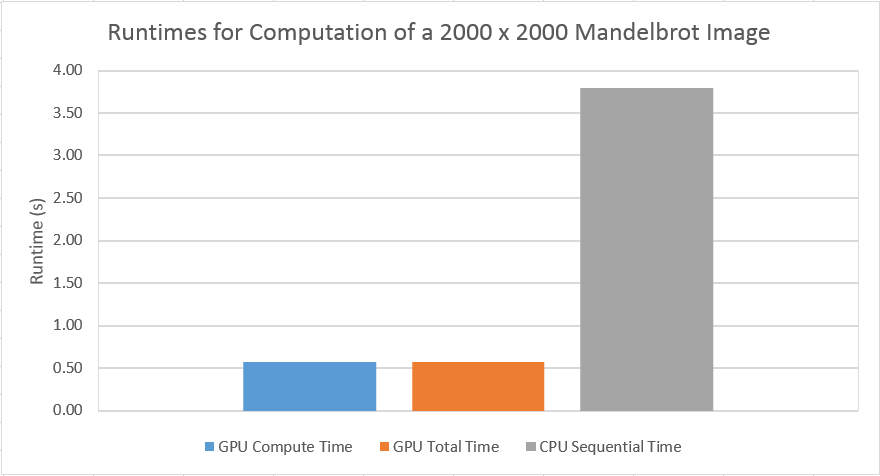
\includegraphics[width=.9\linewidth]{runtime}
    \caption{A comparison of the runtimes for computing a 2000x2000 Mandelbrot image using 1024 iterations at most for each pixel.}
    \label{fig:runtime}
  \end{figure}

  \begin{figure}[h!]
    \centering
    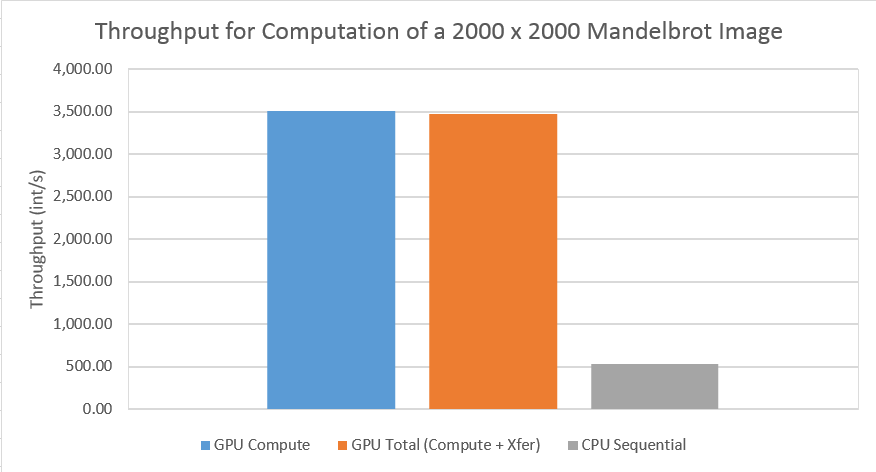
\includegraphics[width=.9\linewidth]{throughput}
    \caption{A comparison of the throughput in integer pixel values produced per second.}
    \label{fig:throughput}
  \end{figure}

  \begin{figure}[h!]
    \centering
    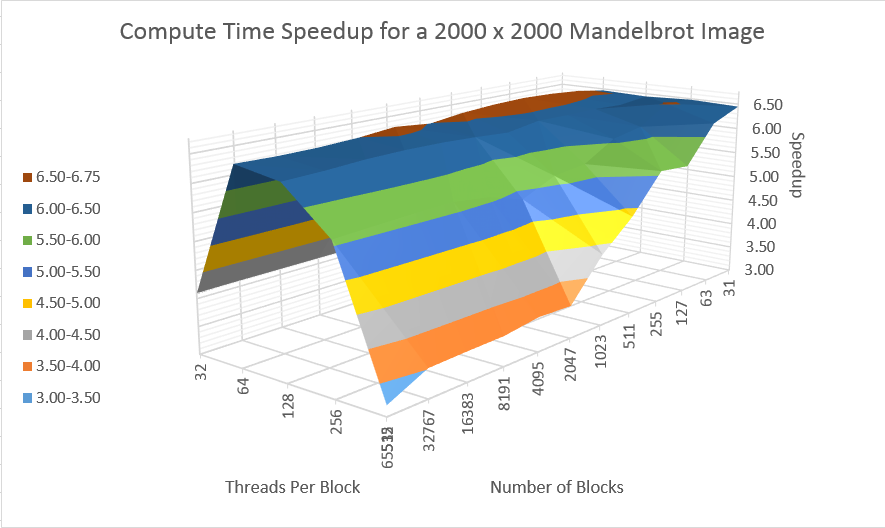
\includegraphics[width=.9\linewidth]{compute_speedup}
    \caption{The speedup achieved. Note the peak in the surface at 64 threads for all block sizes.}
    \label{fig:compute_speedup}
  \end{figure}

  \begin{figure}[h!]
    \centering
    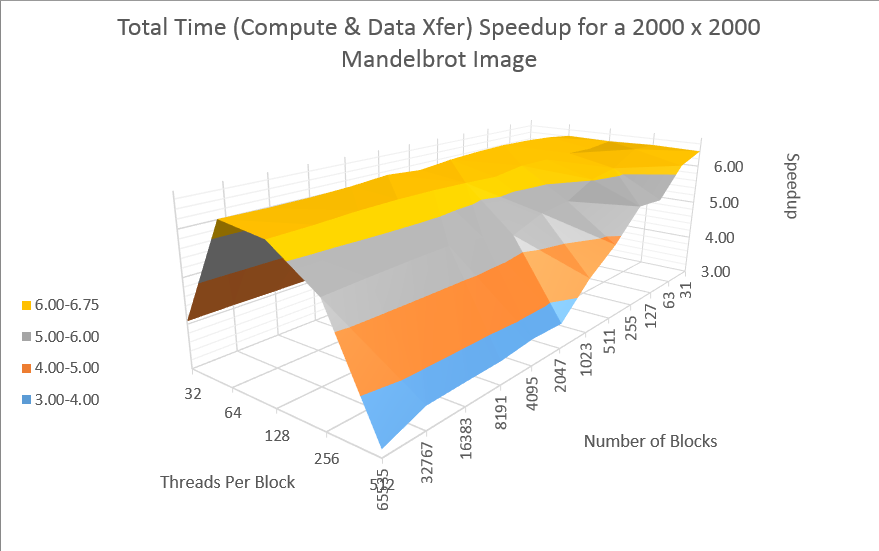
\includegraphics[width=.9\linewidth]{total_speedup}
    \caption{The speedup achieved when also considering the time to copy the computed data from the GPU to the Host.}
    \label{fig:total_speedup}
  \end{figure}

  \begin{figure}[h!]
    \centering
    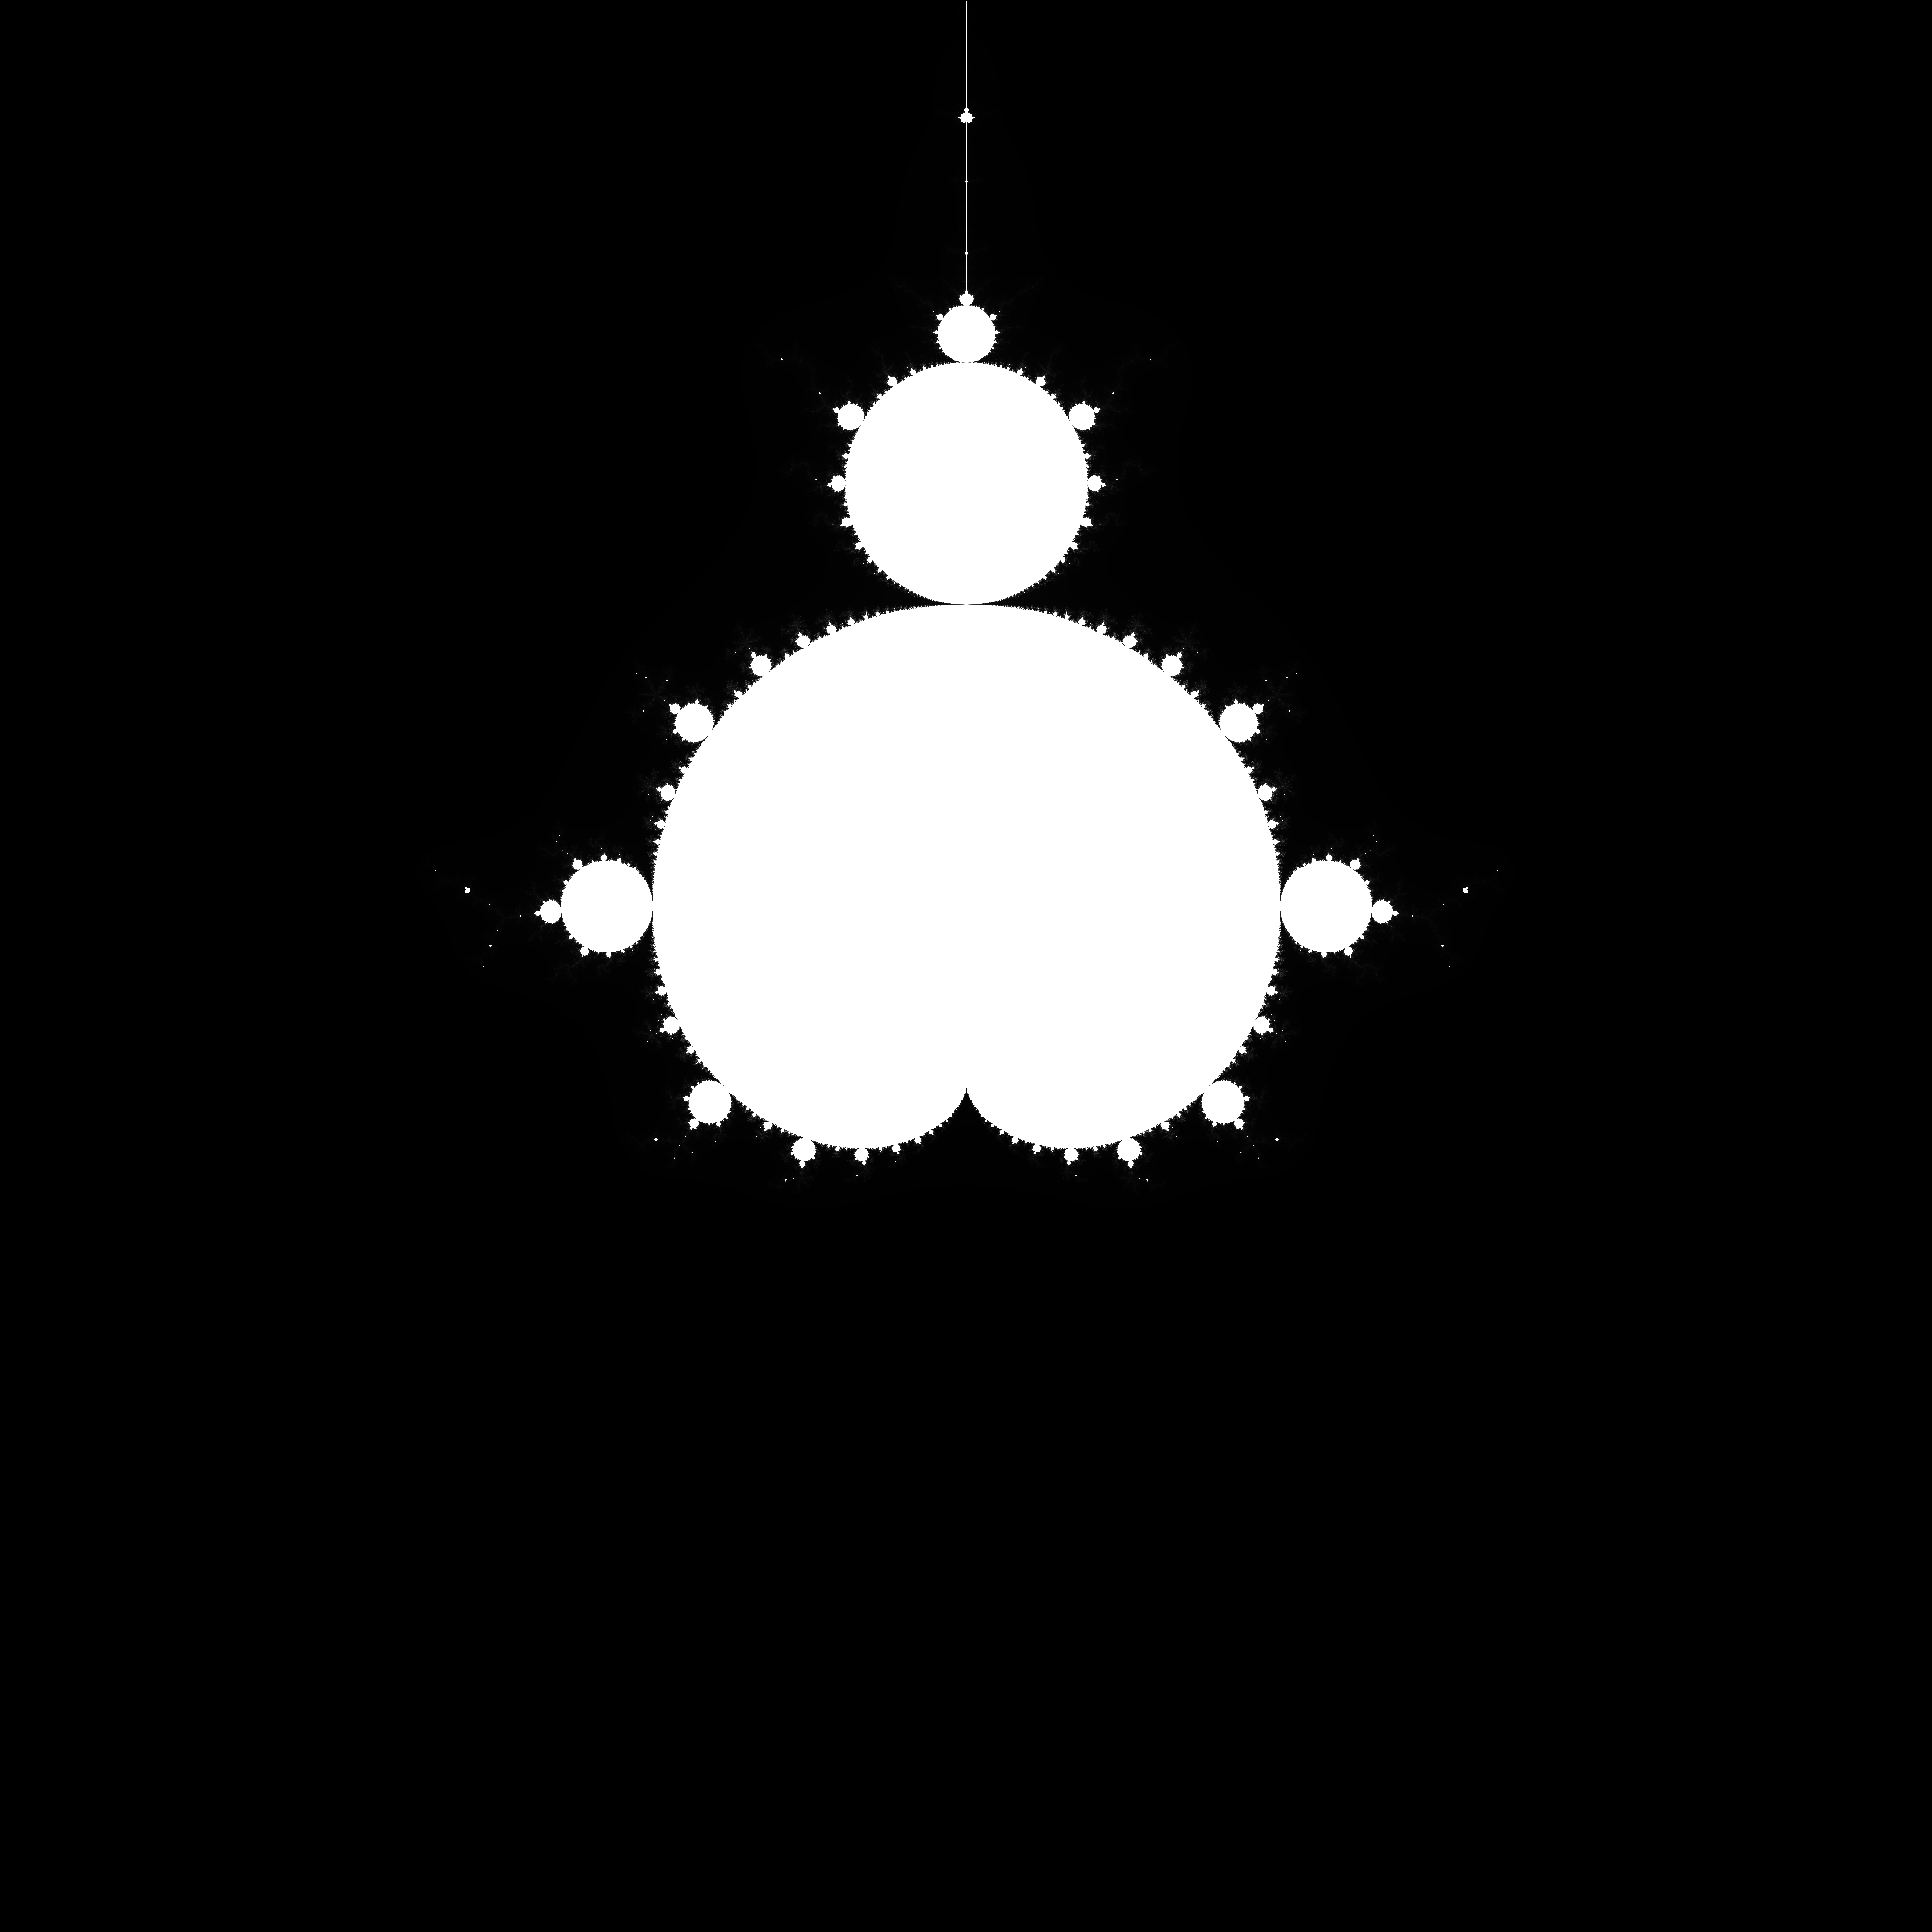
\includegraphics[width=.7\linewidth]{testimage}
    \caption{A Mandelbrot image for verification.}
    \label{fig:total_speedup}
  \end{figure}

\newpage
\section{Discussion}
\subsection{Low Speedups}
The speedups were not as high as I had thought they would be. I believe that this is likely due to my use of a weak GPU - specifically the one that is in my laptop. I have little reason to believe that the lack of speedup was due to a mismatch of algorithms because the sequential and the parallel algorithms are so similar, literally the only difference is the increment factor in the for loop. It is not impressive, but I was able to write CUDA code and do the explorations for the assignment.

\subsection{The Right Number of Threads/Blocks (or The Right ``Stride")}
The highest speedup (for the 2000 x 2000 image) was observed using $255$ blocks $64$ and threads per block to produce a speedup of approximately $6.64$. Looking at the speedup surface graphs do seem to indicate that the number of threads per block was more important than the number of total blocks used. I believe that this is likely because Mandelbrot computation has a high computation to memory access ratio. It is likely that since the threads only need to make $1$ global memory access at the end of their computation, so it is better to keep the number of threads low so that they can spend their time performing the computations.

\subsection{Lack of Transfer Time}
Unlike with many other processes that are parallelized on the GPU, memory transfer time was almost negligible for this task. Only one transfer needs to occur since GPU threads ca figure everything about a pixel out based on which index they are processing

\section{Issues}
\subsection{Weak Hardware Setup}
The GPU used was a medium caliber laptop card. This resulted in limited performance, memory sizes, thread/block counts, etc. In addition, the Windows operating system was used, meaning that all GPU operations needed to occur within $2$ seconds. This limited My data collection from using anything less than 32 threads per block and be able to have consistent success (16 threads worked often, but not often enough). However, I believe enough data was gathered to be able to comprehensively address the topic.
  
\end{document}
